% Deve resumir o experimento, os resultados e a discussão (comentários)
% e incluir opiniões do grupo e propostas futuras para o experimento
%Descrição do hardware
%Descrição do software

\subsection{Descrição do Hardware}\label{hardware}

	Pelo grupo ter escolhido apresentar o experimento utilizando apenas o LCD gráfico, modelo LS020, o único circuito eletrônico acrescentado ao LaunchPad foi o LCD e uma bateria de 9V para alimentação do backlight do display, como pode ser observado na figura \ref{f1}.

\begin{SCfigure}[1][h] %%Cuidado..ela não se mantem no lugar
  \centering
  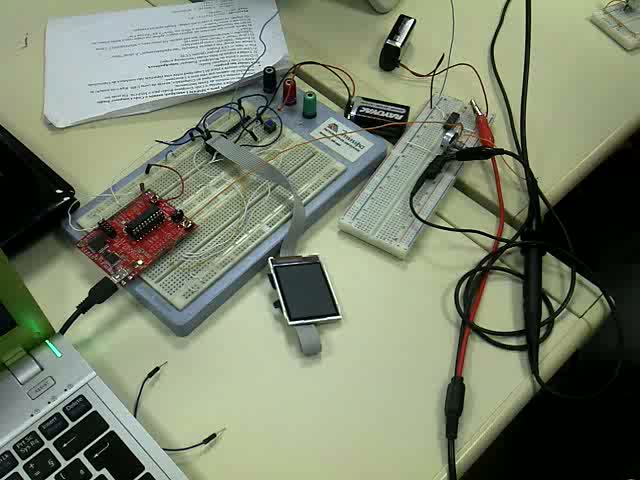
\includegraphics[width=4cm]{./fts/snapshot-001}
  \caption{Vista da protoboard na apresentação final.}
  \label{f1}
\end{SCfigure}



\begin{SCfigure}[1][h] %%Cuidado..ela não se mantem no lugar
  \centering
  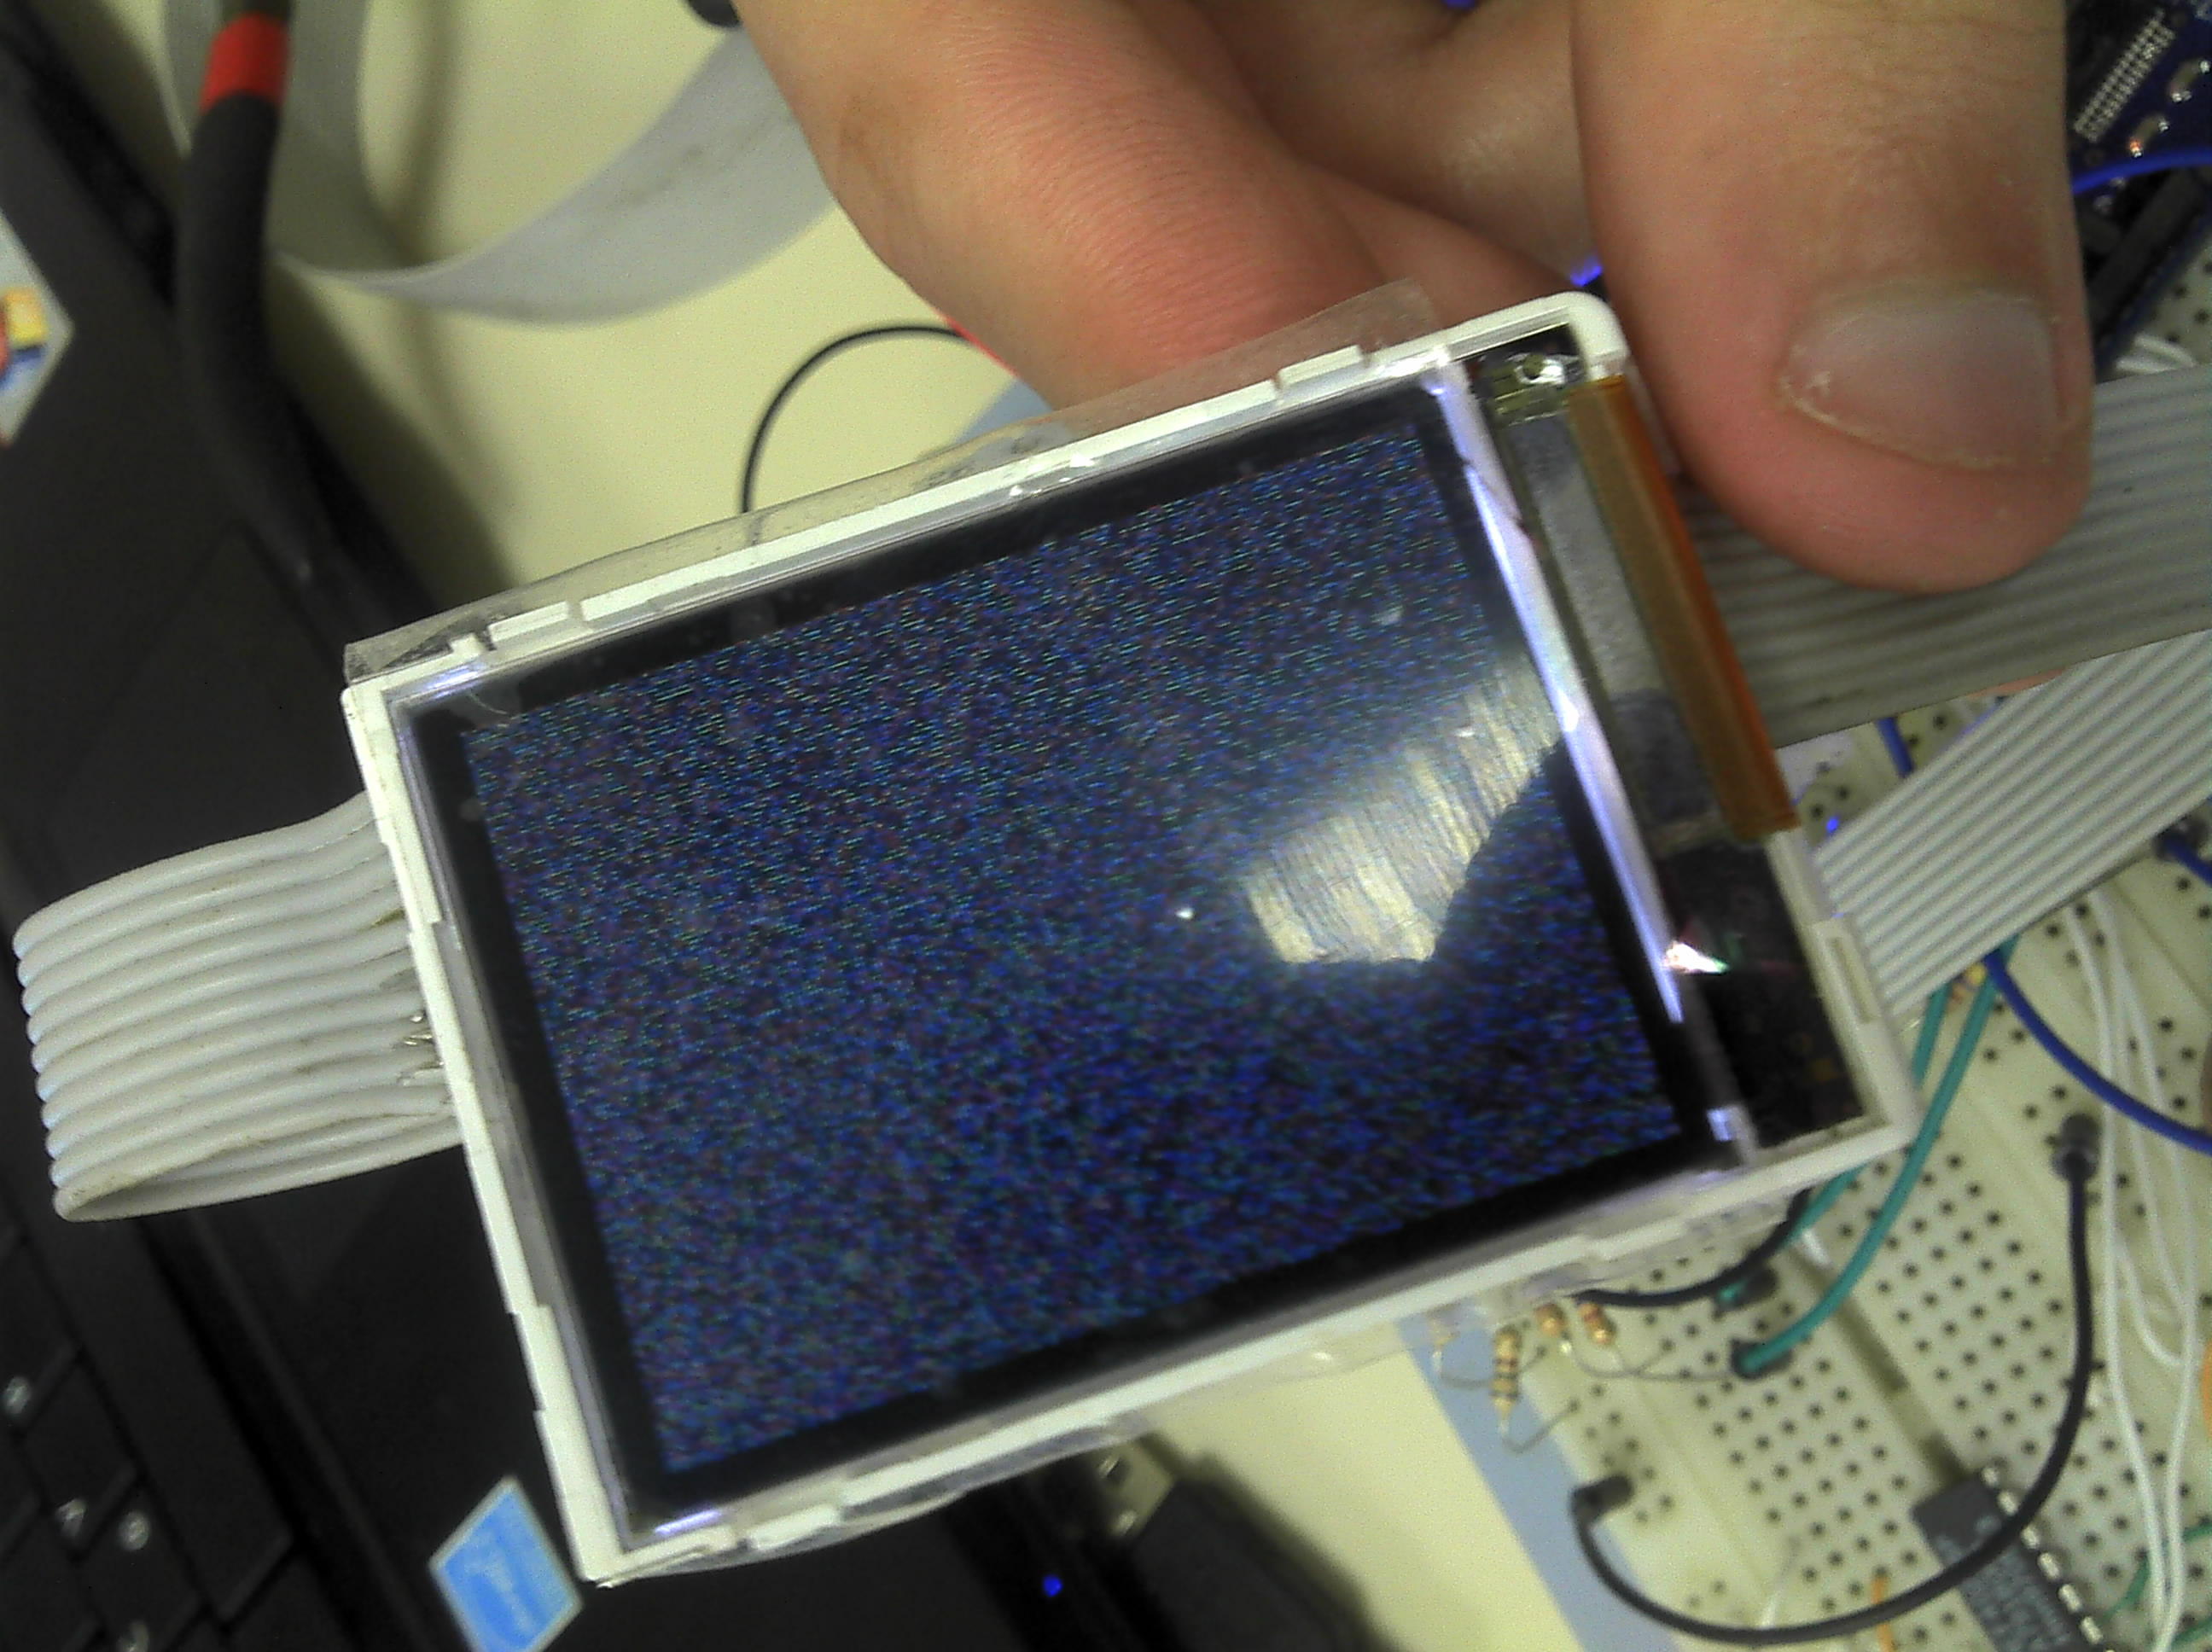
\includegraphics[width=4cm,angle=270]{./fts/f1}
  \caption{Lcd Inicializado.}
  \label{lcd1}
\end{SCfigure}

\subsection{Descrição do Software}\label{software}

Este laboratório teve sem duvidas o código principal mais simples de todos, se desconsiderar todo o código para o funcionamento do LCD. Abaixo encontra-se o arquivo \textit{main.c}, contendo a rotina principal e a interrupção do ADC. Das linhas 11 à 14 o ADC é configurado, habilitado, porém a linha 13 garante que nenhuma amostra será colhida. As linhas 17 e 18 chamas as rotinas para inicializar o LCD (semelhante à figura \ref{lcd1}) e preenche-lo com a cor branca. Em seguida o LED no bit 6 é aceso, representado que o chip esta pronto para inicializar a conversão.

%\lstinputlisting[language=C]{../base.h}
\lstinputlisting[language=C]{../main.c}
%
No laço principal (\textit{while(1)}), a função ploc() é chamada utilizando como parâmetro a variável \textit{ADC10MEM}, que contém o valor atual do ADC. O registrador \textit{ADC10DTC1} é atualizado com 1, para a próxima conversão. Desabilita-se então a interrupção do ADC e espera enquanto o conversor esta ocupado com a conversão. Por fim reconfigura-se o ADC e o coloca em baixo consumo, esperando a próxima colheita. Na interrupção o chip é acordado e é feito um pulso no LED do bit 6. O código teve como  base os exemplos disponibilizados pela Texas Instruments\cite{ti_exemplos}.

\lstinputlisting[language=C]{../ploc.c}

A função ploc é bem simples e apenas plota o valor passado para ela no LCD. Nela é feita a aplicação do filtro, retratado pela equação \ref{filtro}. 

\begin{SCfigure}[1][h] %%Cuidado..ela não se mantem no lugar
  \centering
  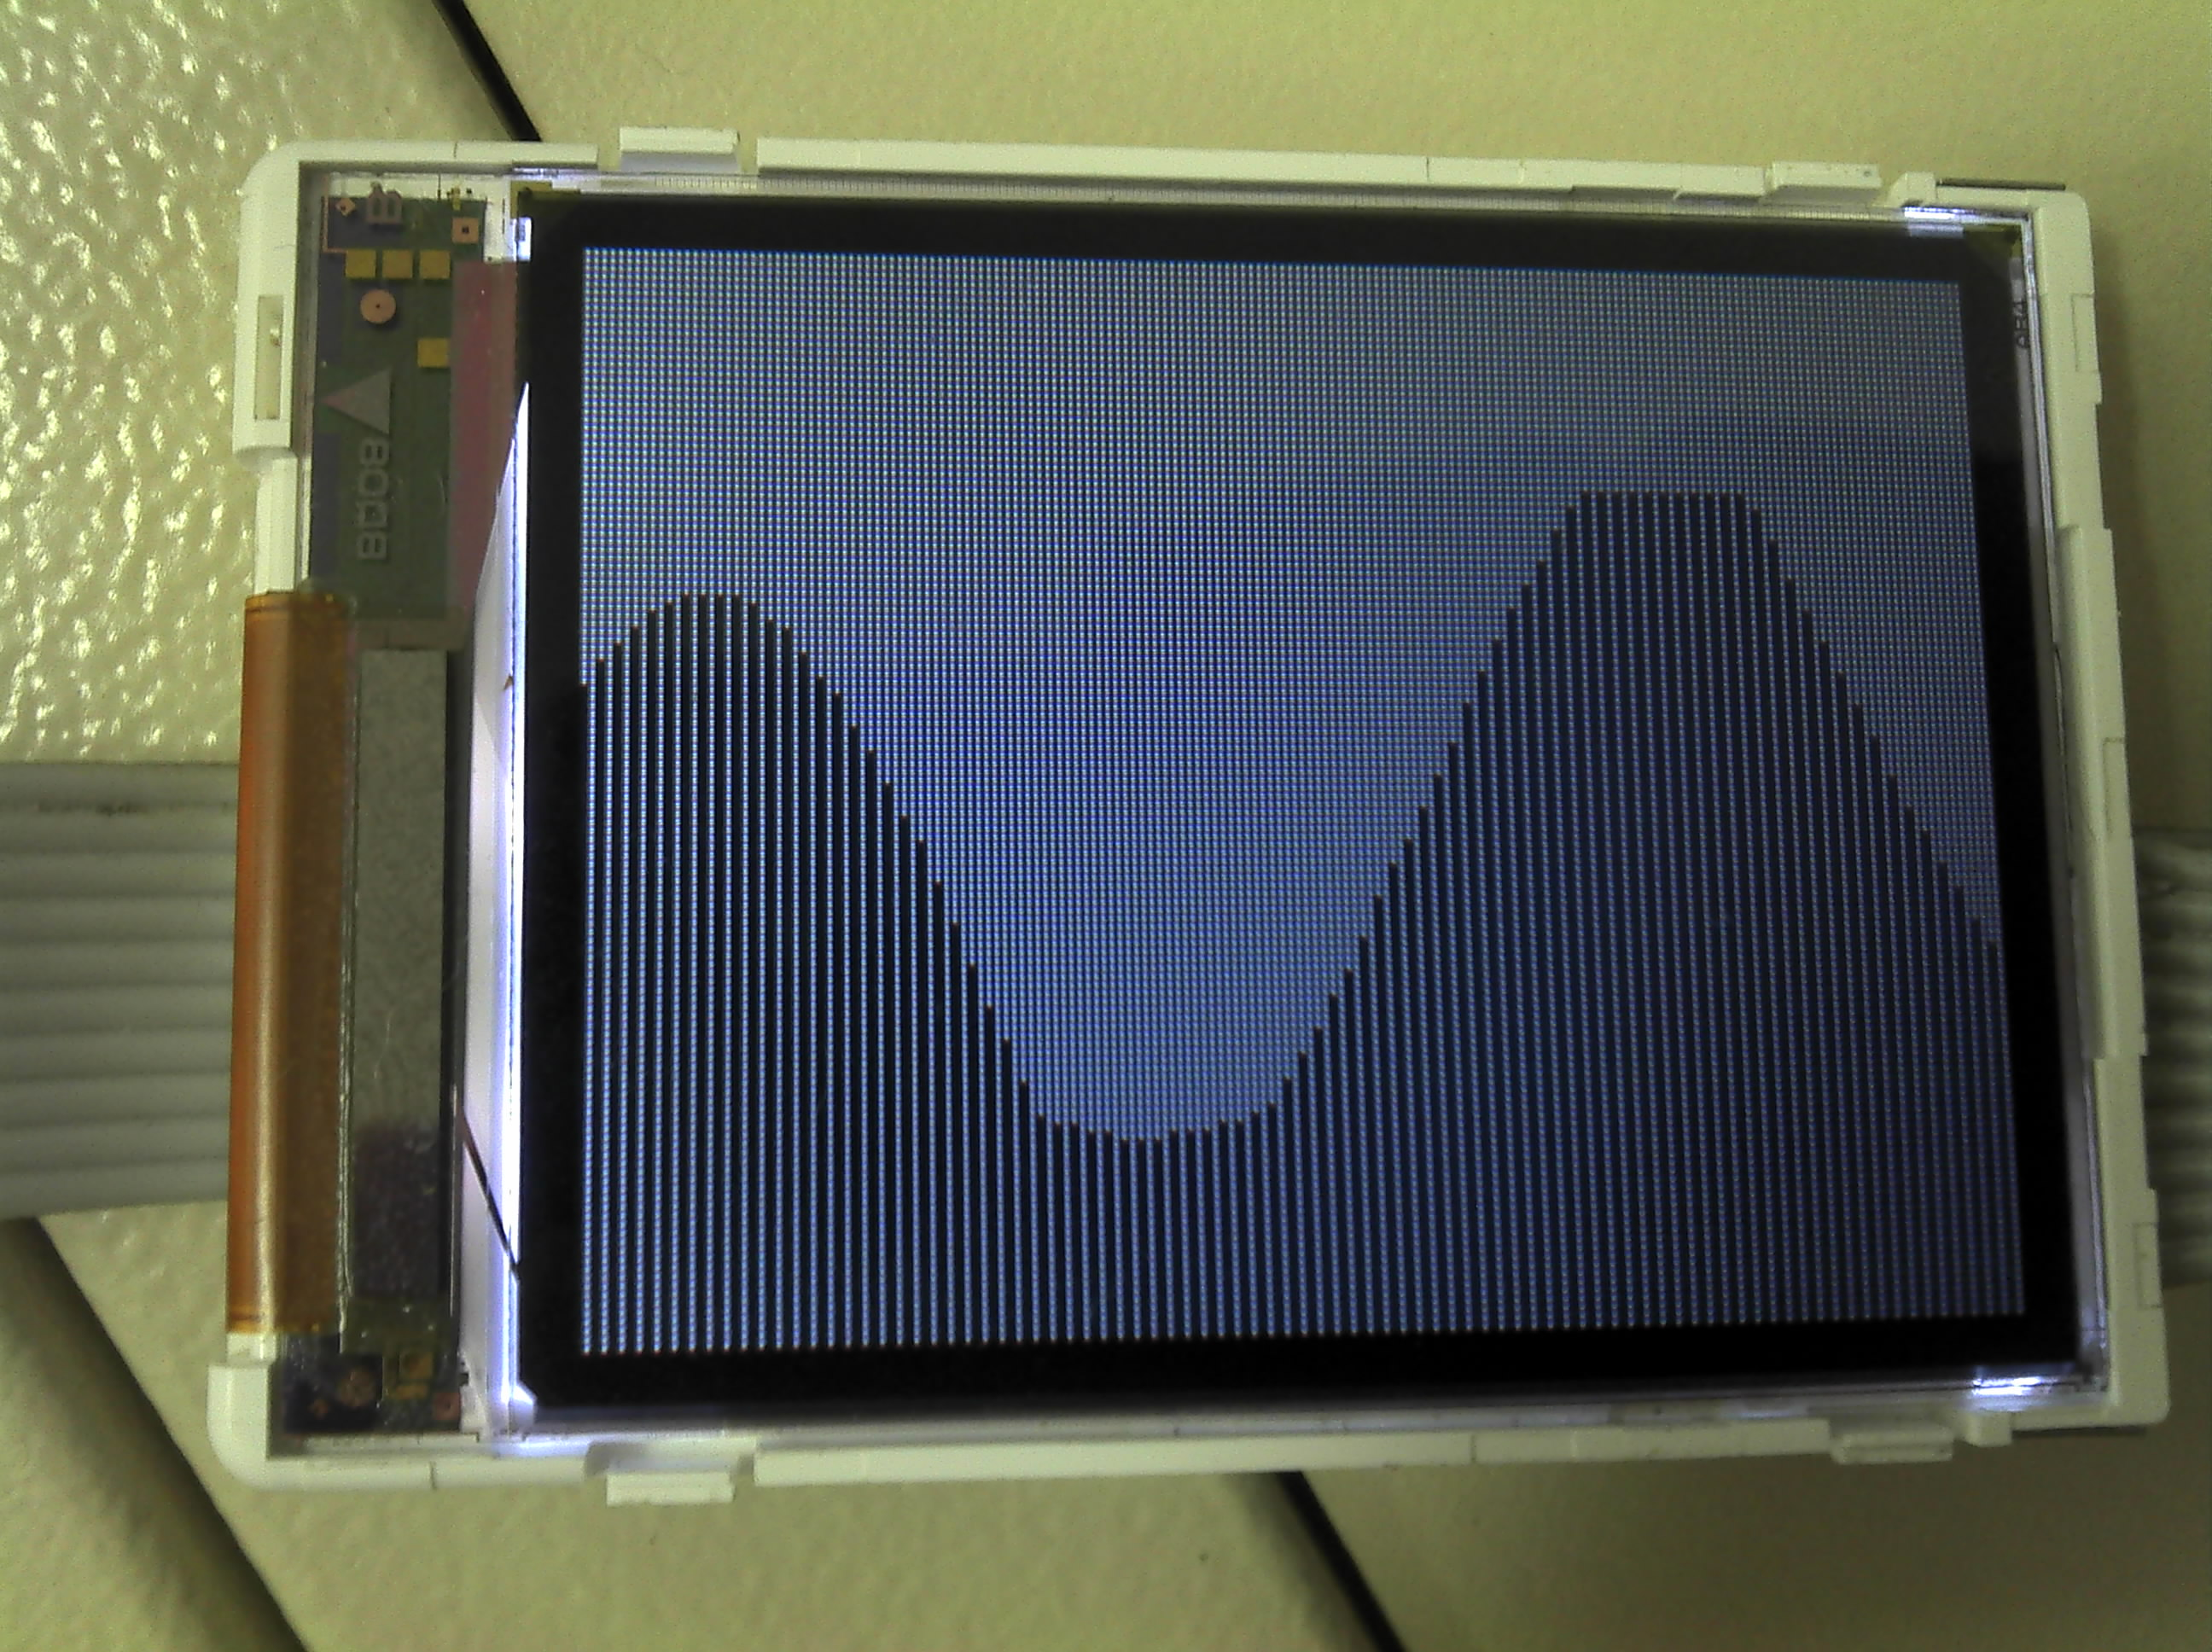
\includegraphics[width=4cm,angle=0]{./fts/snap2}
  \caption{Saída em forma de barras}
  \label{barras}
\end{SCfigure}

Para um maior controle do código, é possivel alterar a saída via código, definindo ou não a macro \textit{\_\_GRAFICO\_BARRAS\_\_} para alterar a saída do display de linhas (figura \ref{linhas}) ou barras (figura \ref{barras}).

\begin{SCfigure}[1][h] %%Cuidado..ela não se mantem no lugar
  \centering
  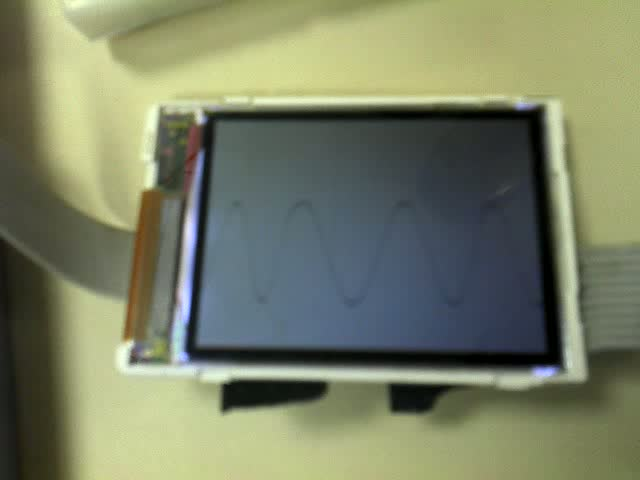
\includegraphics[width=4cm,angle=0]{./fts/snap0}
  \caption{Saída em forma de linhas}
  \label{linhas}
\end{SCfigure}

%\lstinputlisting[language=MSP430]{../prog.asm}
